\chapter{Multiple Integral} \label{ch7ch}

The integral for scalar input function has been introduced in Chapter \ref{ch3}. The integral of $y=f(x)$ with the lower bound $a$ and upper bound $b$ is denoted by \eqref{ch3eq:generaldefiniteintegral2}. It is defined as the limit of sum given by \eqref{ch3eq:generaldefiniteintegral}, and can be interpreted as the area circulated by $x=a$, $x=b$, $y=f(x)$ and $y=0$ as shown by Fig. \ref{ch3fig:explainintegrial}. In practice, the integral can be calculated using \eqref{ch3eq:calculatedefiniteintegral}.

In this chapter, the integral for multiple input functions is introduced. Motivating examples are used to illustrate the basic concept and meaning of multiple integral in Section \ref{ch7sec:motivatingexp}. The formal definition of multiple integral is given in Section \ref{ch7sec:multipleintegral}.

\section{Motivating Examples} \label{ch7sec:motivatingexp}

\begin{shortbox}
\Boxhead{Motivating Example 1}

Consider calculating the volume of a cone using integral. The bottom radius and the height of the cone are $1$ and $3$ respectively.

\end{shortbox}

Figure \ref{ch7fig:motivatingexp1} gives a demonstration of the cone in the motivating example. Using similar ideas introduced in Chapter \ref{ch3}, we know that we can think of the cone as a combination of thin cylinders, whose radiuses depend on the vertical position ($z$-axis position) of the associated cylinder. For example, at $z=1.5$, the radius of the cylinder is $0.5$.

\begin{figure}
	\centering
	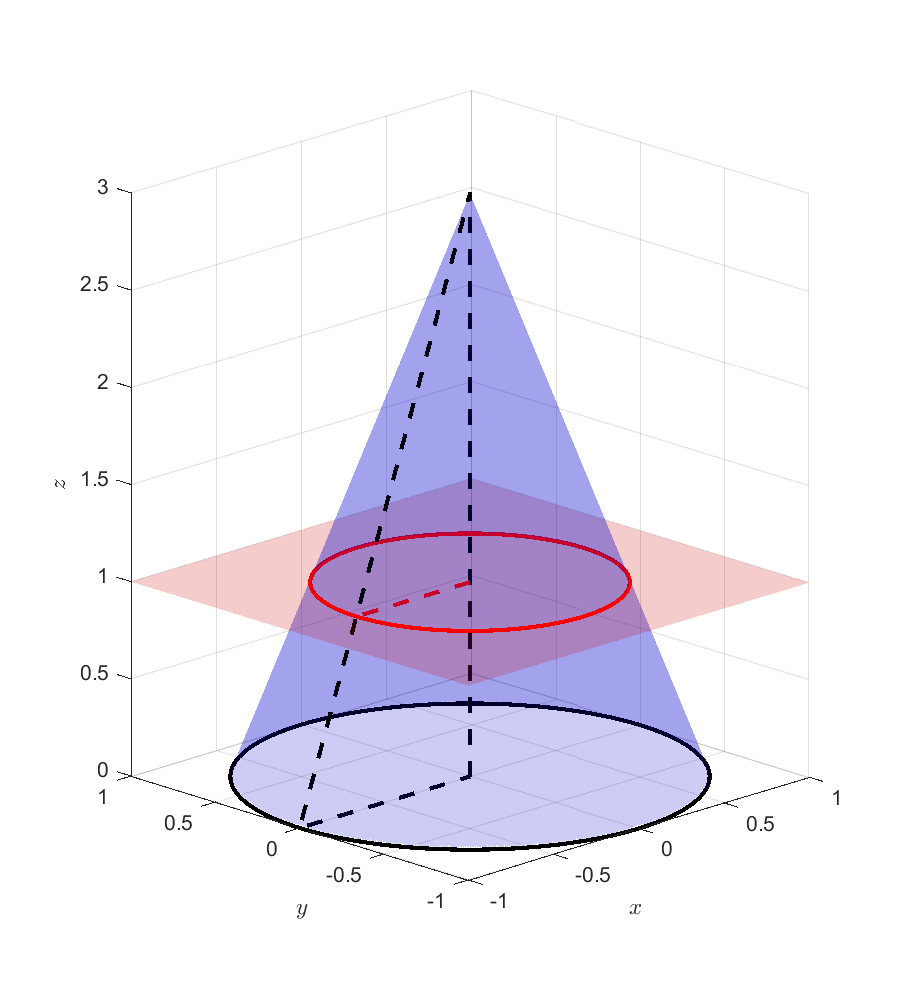
\includegraphics[width=200pt]{chapters/chapter7/figures/motivatingexp1.eps}
	\caption{Calculation of the volume of a cone.} \label{ch7fig:motivatingexp1}
\end{figure}

The volume of the cone can be obtained by letting the thickness of each cylinder approaches zero. i.e.,
\begin{eqnarray}
  V &=& \int_{0}^{3}S(z)dz, \label{ch7eq:motivatingv} \\
  S(z) &=& \pi R(z)^2, \label{ch7eq:motivatingsz} \\
  R(z) &=& \dfrac{3-z}{3}, 0\leq z\leq 3, \label{ch7eq:motivatingrz} 
\end{eqnarray}
where $R(z)$ and $S(z)$ are the bottom circle radius and area of the thin cylinder at vertical position $z$, and $S(z)dz$ can be interpreted as the volume of this thin cylinder. 

Substituting \eqref{ch7eq:motivatingsz} and \eqref{ch7eq:motivatingrz} into \eqref{ch7eq:motivatingv} gives
\begin{eqnarray}
  V = \int_{0}^{3} \dfrac{\pi}{9} \left(3-z\right)^2 dz 
  = \left.\dfrac{\pi}{27}(z-3)^3 \right|_0^3 
  = \pi \nonumber
\end{eqnarray}
which is consistent with what we learned in primary school: the volume of a cone is one third of its bottom area multiplied by its height.


\section{Multiple Integral} \label{ch7sec:multipleintegral}

